\documentclass[letterpaper,12pt]{article}
\usepackage{array}
\usepackage{threeparttable}
\usepackage{geometry}
\geometry{letterpaper,tmargin=1in,bmargin=1in,lmargin=1.25in,rmargin=1.25in}
\usepackage{fancyhdr,lastpage}
\pagestyle{fancy}
\lhead{}
\chead{}
\rhead{}
\lfoot{}
\cfoot{}
\rfoot{\footnotesize\textsl{Page \thepage\ of \pageref{LastPage}}}
\renewcommand\headrulewidth{0pt}
\renewcommand\footrulewidth{0pt}
\usepackage[format=hang,font=normalsize,labelfont=bf]{caption}
\usepackage{listings}
\usepackage{color}
\definecolor{dkgreen}{rgb}{0,0.6,0}
\definecolor{gray}{rgb}{0.5,0.5,0.5}
\definecolor{mauve}{rgb}{0.58,0,0.82}
\lstset{ %
  language=R,                     % the language of the code
  basicstyle=\footnotesize,       % the size of the fonts that are used for the code
  numbers=left,                   % where to put the line-numbers
  numberstyle=\tiny\color{gray},  % the style that is used for the line-numbers
  stepnumber=1,                   % the step between two line-numbers. If it's 1, each line
  numbersep=5pt,                  % how far the line-numbers are from the code
  backgroundcolor=\color{white},  % choose the background color. You must add \usepackage{color}
  showspaces=false,               % show spaces adding particular underscores
  showstringspaces=false,         % underline spaces within strings
  showtabs=false,                 % show tabs within strings adding particular underscores
  frame=single,                   % adds a frame around the code
  rulecolor=\color{black},        % if not set, the frame-color may be changed on line-breaks within not-black text (e.g. commens (green here))
  tabsize=2,                      % sets default tabsize to 2 spaces
  captionpos=b,                   % sets the caption-position to bottom
  breaklines=true,                % sets automatic line breaking
  breakatwhitespace=false,        % sets if automatic breaks should only happen at whitespace
  title=\lstname,                 % show the filename of files included with \lstinputlisting;
  keywordstyle=\color{blue},      % keyword style
  commentstyle=\color{dkgreen},   % comment style
  stringstyle=\color{mauve},      % string literal style
  escapeinside={\%*}{*)},         % if you want to add a comment within your code
  morekeywords={*,...}            % if you want to add more keywords to the set
}
\usepackage{amsmath}
\usepackage{amssymb}
\usepackage{amsthm}
\usepackage{harvard}
\usepackage{setspace}
\usepackage{float,color}
\usepackage[pdftex]{graphicx}
\usepackage{hyperref}
\hypersetup{colorlinks,linkcolor=red,urlcolor=blue}
\theoremstyle{definition}
\newtheorem{theorem}{Theorem}
\newtheorem{acknowledgement}[theorem]{Acknowledgement}
\newtheorem{algorithm}[theorem]{Algorithm}
\newtheorem{axiom}[theorem]{Axiom}
\newtheorem{case}[theorem]{Case}
\newtheorem{claim}[theorem]{Claim}
\newtheorem{conclusion}[theorem]{Conclusion}
\newtheorem{condition}[theorem]{Condition}
\newtheorem{conjecture}[theorem]{Conjecture}
\newtheorem{corollary}[theorem]{Corollary}
\newtheorem{criterion}[theorem]{Criterion}
\newtheorem{definition}[theorem]{Definition}
\newtheorem{derivation}{Derivation} % Number derivations on their own
\newtheorem{example}[theorem]{Example}
\newtheorem{exercise}[theorem]{Exercise}
\newtheorem{lemma}[theorem]{Lemma}
\newtheorem{notation}[theorem]{Notation}
\newtheorem{problem}[theorem]{Problem}
\newtheorem{proposition}{Proposition} % Number propositions on their own
\newtheorem{remark}[theorem]{Remark}
\newtheorem{solution}[theorem]{Solution}
\newtheorem{summary}[theorem]{Summary}
%\numberwithin{equation}{section}
\bibliographystyle{aer}
\newcommand\ve{\varepsilon}
\newcommand\boldline{\arrayrulewidth{1pt}\hline}


\begin{document}

\begin{flushleft}
  \textbf{\large{Problem Set \#4}} \\
  MACS 30100, Dr. Evans \\
  Cheng Yee Lim
\end{flushleft}

\vspace{5mm}

\noindent\textbf{Problem 1}\\
\textbf{Part (a).}
\begin{figure}[htb]\centering\captionsetup{width=4.0in}
  \caption{\textbf{Normed Histogram of Percentages of income}}\label{FigExample}
  \fbox{\resizebox{6.0in}{4.0in}{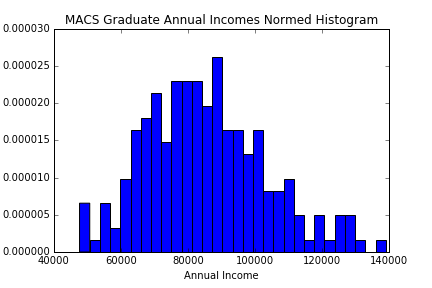
\includegraphics{images/1a.png}}}
\end{figure}

\pagebreak
\flushleft
\textbf{Part (b).} \\

\flushleft 
The function for the lognormal PDF is $LN\textunderscore pdf(xvals, \mu, \sigma)$. \\
The output of $LN\textunderscore pdf(np.array([200.0, 270.0], [180.0, 195.5]), 5.0, 1.0)$ is 
\[
M_1 =
  \begin{bmatrix}
		0.0019079 & 0.00123533 \\
		0.00217547 & 0.0019646
  \end{bmatrix}
\]

\textbf{Part (c)} \\
The estimated $\mu_{1c}$ is 11.3307606999 and the estimated $\sigma_{1c}$ is 0.209202916466.\\
The SMM criterion function is $1.40124304\times10^{-8}$.\\
The mean and standard deviation of data moments are \\85276.82360625811 and 17992.542128046523.\\
The mean and standard deviation of model moments are \\85286.87240412165 and 17992.33953712455.\\
Despite using an identity matrix as the weighting matrix, the data and model moments are highly similar. In fact the mean data and model moment are identical to 3 significant factors and the standard deviation moment are identical to 5 significant factors. The highly similar data and model moments show that the SMM estimation was a good estimation. 
\begin{figure}[htb]\centering\captionsetup{width=4.0in}
  \caption{\textbf{Normed Histogram of MACSS Students Annual Income and the SMM Log PDF}}\label{FigExample}
  \fbox{\resizebox{6.0in}{4.0in}{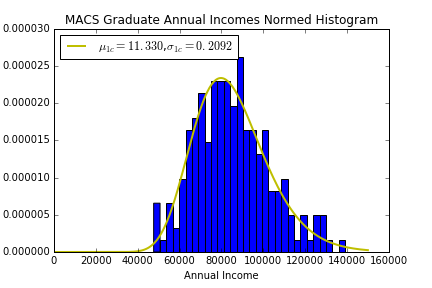
\includegraphics{images/1c.png}}}
\end{figure}

\pagebreak
\textbf{Part (d).} \\
\flushleft 
\begin{figure}[htb]\centering\captionsetup{width=4.0in}
  \caption{\textbf{Normed histogram of Annual Incomes of MACSS Graduates and 2-step Weight Matrix LogNormal PDF}}\label{FigExample}
  \fbox{\resizebox{6.0in}{4.0in}{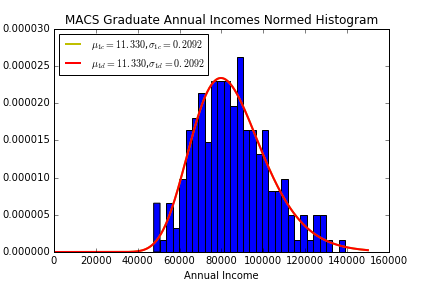
\includegraphics{images/1d.png}}}
\end{figure}

The SMM estimates for $\mu_{1d}$ and $\sigma_{1d}$ are 11.3307606999 and 0.209202916466.\\ 
The SMM criterion function is $1.40124304\times10^{-8}$.\\
The mean and standard deviation of data moments are\\ 85276.82360625811 and 17992.542128046523.\\
The mean and standard deviation of modelled moments are \\85286.87240412165 and 17992.33953712455.\\
Expectedly, the results of the two step variance covariance weights matrix SMM estimation are highly similar to the data moments. However, since the estimation in part (c) was already close to perfect, a marked improvement could not be seen comparing part (d) to (c) as both estimations were good estimations. 

\end{document}
